
\documentclass[conference,letterpaper]{IEEEtran}
\setlength{\pdfpagewidth}{8.5in}

\setlength{\pdfpageheight}{11in}

\usepackage{graphicx}
\usepackage{caption}
\usepackage{subcaption}
%\usepackage{subfigure}
\usepackage{textcomp}
\usepackage{hyperref}
\hypersetup{pdfpagemode=UseNone}
%\usepackage{subfig}
\usepackage{booktabs}
\usepackage{multirow}
%\usepackage{natbib}
\usepackage{color,soul}
\let\labelindent\relax
\usepackage{enumitem}
\usepackage{balance}

%\usepackage{amsmath,scalerel}

%\DeclareMathOperator*{\Bigcdot}{\scalerel*{\cdot}{\bigodot}}

\newtheorem{cond}{Condition}
\newtheorem{defn}{Definition}

\usepackage{etoolbox}

\usepackage{microtype}

\usepackage{fixltx2e}

\usepackage[numbers,sort&compress]{natbib}

\usepackage[table]{xcolor}


%command to comment out stuff
\newcommand{\comment}[1]{}

%-----------------------------------------------------
%space saving!!!
\newcommand{\abovesectitle}{0pt}
\newcommand{\undersectitle}{0pt}
\newcommand{\abovesubsectitle}{0pt}
\newcommand{\undersubsectitle}{0pt}
\newcommand{\abovesubsubsectitle}{0pt}
\newcommand{\undersubsubsectitle}{0pt}
\newcommand{\abovesubsubcancel}{0pt}
%\comment{
\addtolength{\textfloatsep}{-17pt}
\addtolength{\floatsep}{-7pt}
\addtolength{\abovecaptionskip }{-4pt}
\addtolength{\dbltextfloatsep}{-13pt}
\addtolength{\dblfloatsep}{-5pt}

%Change caption size to small
\renewcommand{\captionfont}{\small}
\renewcommand{\captionlabelfont}{\small}

%Spacing before and after sub/section
\renewcommand{\abovesectitle}{-4pt}
\renewcommand{\undersectitle}{-4pt}
%
\renewcommand{\abovesubsectitle}{-6pt}
\renewcommand{\undersubsectitle}{-3pt}
%
\renewcommand{\abovesubsubsectitle}{-5pt}
\renewcommand{\undersubsubsectitle}{-2pt}
\renewcommand{\abovesubsubcancel}{5pt}

%reduce space between bib entries -- requires natbib
%\setlength{\bibsep}{0.04cm}

%use 0.95 or higher
\linespread{0.92}

\setlist[itemize]{leftmargin=*}
\setlist[enumerate]{leftmargin=*}
%}
%-----------------------------------------------------



\begin{document}
%\makeatletter
%\patchcmd{\@afterheading}%
%    {\clubpenalty \@M}{\clubpenalties 3 \@M \@M 0}{}{}
%\patchcmd{\@afterheading}%
%    {\clubpenalty \@clubpenalty}{\clubpenalties 2 \@clubpenalty 0}{}{}
%\makeatother
\sloppy
%


%--------------------------------------------------------------------------------------------
% Custom commands
%--------------------------------------------------------------------------------------------

%\renewcommand{\footnoterule}{%
%  \kern -3pt
%  \hrule width 0.49\textwidth height 0.5pt
%  \kern 2pt
%} 

\newcommand{\til}{{\fontfamily{ptm}\selectfont\texttildelow}}
\newcommand{\xx}{$\times${ }}

%shortcut command for pdf figures
\newcommand{\fig}[3]{\begin{figure}[t]
\centering
\includegraphics[width=2.5in,#2]{figs/#1}
\caption{#3}
\label{#1}
\end{figure}}

%shortcut command for pdf figures
\newcommand{\figg}[4]{\begin{figure}[t]
\centering
\includegraphics[width=#2,#3]{figs/#1}
\caption{#4}
\label{#1}
\end{figure}}

%shortcut command for pdf figures
\newcommand{\figc}[3]{\begin{figure}[t]
\centering
\includegraphics[width=1.0\columnwidth,keepaspectratio,#2]{figs/#1}
\caption{#3}
\label{#1}
\end{figure}}

%shortcut command for pdf figures
\newcommand{\figch}[3]{\begin{figure}[h]
\centering
\includegraphics[width=1.0\columnwidth,keepaspectratio,#2]{figs/#1}
\caption{#3}
\label{#1}
\end{figure}}


%shortcut command for pdf figures
\newcommand{\figvs}[4]{\begin{figure}[!t]
\centering
\includegraphics[width=#1\columnwidth,keepaspectratio,#3]{figs/#2}
\caption{#4}
\label{#2}
\end{figure}}

%shortcut command for pdf figures
\newcommand{\figvsh}[4]{\begin{figure}[!h]
\centering
\includegraphics[width=#1\columnwidth,keepaspectratio,#3]{figs/#2}
\caption{#4}
\label{#2}
\end{figure}}


%shortcut command for pdf figures
\newcommand{\figfull}[4]{\begin{figure*}[!t]
\centering
\includegraphics[width=#1\columnwidth,keepaspectratio,#3]{figs/#2}
\caption{#4}
\label{#2}
\end{figure*}}

%shortcut command for pdf figures with placement hint
\newcommand{\figp}[4]{\begin{figure}[#4]
\centering
\includegraphics[width=2.5in,#2]{figs/#1}
\caption{#3}
\label{#1}
\end{figure}}

%adding subsubsubsection
\newcommand{\subsubsubsection}[1]{\vspace{0.2cm}\noindent\textbf{\textit{#1:}}}



%--------------------------------------------------------------------------------------------
% Title
%--------------------------------------------------------------------------------------------

\title{Bringing Programmability to the Data Plane: \\ Packet Processing with a NoC-Enhanced FPGA} 

%\subtitle{--blind submission--}


% author names and affiliations
% use a multiple column layout for up to three different
% affiliations
\author{\IEEEauthorblockN{Andrew Bitar, Mohamed S. Abdelfattah, Vaughn Betz}
\IEEEauthorblockA{Department of Electrical and Computer Engineering\\
University of Toronto, Toronto, ON, Canada\\
\{bitar, mohamed, vaughn\}@eecg.utoronto.ca}
}

%\author{-blinded-}



\maketitle


%
%#############################################################
% ABSTRACT
%-0-0-0-0-0-0-0-0-0-0-0-0-0-0-0-0-0-0-0-0-0-0-0-0-0-0-0-0-0-0-
%
\begin{abstract}
%
%
\comment{
\hl{change abstract to reflect new material}
Embedded logic and I/O interfaces have made field-programmable gate-arrays (FPGAs) more capable platforms for implementing large systems.
We explore the addition of a fast embedded network-on-chip (NoC) to augment the FPGA's existing wires and switches, and help interconnect large applications.
A flexible interface between the FPGA fabric and the embedded NoC allows modules of varying widths and frequencies to transport data over the NoC.
We study both latency-insensitive and latency-sensitive design styles and present the constraints for implementing each type of communication on the embedded NoC.
%
%
By augmenting field-programmable gate-arrays (FPGAs) with embedded computation, memory and I/O elements, they have become an efficient platform for compute acceleration and networking applications.
However, implementing on-chip communication is still a designer's burden where custom system-level communication buses are implemented using the fine-grained FPGA logic and interconnect fabric.
We propose augmenting FPGAs with an embedded network-on-chip (NoC) to implement system-level communication.
We design custom interfaces to connect a conventional packet-switched NoC to the FPGA fabric and I/Os in a configurable and efficient way.
We then define the necessary rules and constraints to implement FPGA design styles correctly and efficiently using an embedded NoC -- this lays the foundations upon which we can implement applications using a NoC-enhanced FPGA.
In the second half of this paper, we present four application case studies that highlight the advantages of using an embedded NoC.
We show that access-latency to external memory can be \til1.5\xx lower.
Our application case study with image compression shows that an embedded NoC improves frequency by 10--80\%, reduces utilization of scarce long wires by 40\% and makes design easier and more predictable.
Additionally, we leverage the embedded NoC in creating a programmable Ethernet switch that can support up to 819~Gb/s compared to previous work that only demonstrated 160~Gb/s.
Finally we design a 400~Gb/s packet processor based on our embedded NoC, that is more flexible and efficient compared to other packet processor designs.
}
%
%By augmenting field-programmable gate-arrays (FPGAs) with embedded computation, memory and I/O elements, they have become an efficient platform for compute acceleration and networking applications.
Field-programmable gate-arrays (FPGAs) have evolved to include embedded memory, high-speed I/O interfaces and processors, making them both more efficient and easier-to-use for compute acceleration and networking applications.
However, implementing on-chip communication is still a designer's burden wherein custom system-level buses are implemented using the fine-grained FPGA logic and interconnect fabric.
Instead, we propose augmenting FPGAs with an embedded network-on-chip (NoC) to implement system-level communication.
We design custom interfaces to connect a packet-switched NoC to the FPGA fabric and I/Os in a configurable and efficient way and then define the necessary conditions to implement common FPGA design styles with an embedded NoC.
Four application case studies highlight the advantages of using an embedded NoC.
We show that access latency to external memory can be \til1.5\xx lower.
Our application case study with image compression shows that an embedded NoC improves frequency by 10--80\%, reduces utilization of scarce long wires by 40\% and makes design easier and more predictable.
Additionally, we leverage the embedded NoC in creating a programmable Ethernet switch that can support up to 819~Gb/s -- 5\xx more switching bandwidth and 3\xx lower area compared to previous work.
Finally, we design a 400~Gb/s NoC-based packet processor that is very flexible and more efficient than other FPGA-based packet processors.
%

\end{abstract}
%
%
%
%#############################################################
\vspace{\abovesectitle}
\section{Introduction}
\vspace{\undersectitle}
%-0-0-0-0-0-0-0-0-0-0-0-0-0-0-0-0-0-0-0-0-0-0-0-0-0-0-0-0-0-0-
%
%
%
\comment{
\begin{itemize}
	\item outline our previous study of NoCs - what are the efficiency gains that we get.
	\item say that a big question remains unanswered: how do we actually design using that NOC.
	\item we need to know what guarantees can we make? how does it fit in FPGA design? what guarantees can we make? how to simulate designs efficiently?
	\item previous work shows that a full-featured NoC can (1) reduce area/power consumption on FPGAs (2) simplify design especially timing closure because interconnects aren't scaling that well anymore.
	\item scarcely have people looked into how to interface an embedded hard NoC to the FPGA fabric -- we study this in detail and present the designs for a "FabricPort" that interfaces the two.
	\item we also discuss how a full-featured packet-switched NoC (1\% of FPGA area) can be adapted to specifically cater to FPGA designs, why other forms of system-interconnect may not be as suitable.
	\item discuss VCs, VC facilitator, routing algos, buffer sizing.
	\item dally and towles identify two main uses of NoCs as (1) processor-memory communication: this is basically moving cache lines in a homogeneous or heterogenous memory-mapped system, or (2) switch fabric where an NoC acts as one big router.
	\item however, FPGAs aren't typically used for memory-mapped communication, rather streaming data. Stream in --> processing --> stream out. examples are video/internet/packet/data-center/communications.
	\item little or no previous work has looked into using NoCs for implementing streaming data. 
	\item we also show that both latency-sensitive and latency-insenstive communicaiton can be mapped onto an NoC with predictable performance for the former type of interconnect.
	\item we present a cycle-accurate simulation framework for NoCs to test applications with NoC as interconnect and measure latency/throughput performance.
	\item we then present two (or more) applications and compare various metrics both when on or off the NoC.
	\item applications are (1) switch fabric (2) latency-sensitive jpeg (3) latency-insensitive memory access
\end{itemize}

\hl{can compare to previous bus-based FPGA interconnect that didnt really take off -- how are we different and why is our solution better/more flexible.}

%test citations
Previous work has evaluated the area and energy efficiency gains of using embedded NoCs compared to building soft interconnect from the FPGA fabric~\cite{fpl,fpt,trets,micro}.

\hl{the NoC is a new kind of FPGA interconnect resource that provides pipelining, switching, buffering and stallability. Try to convey this idea. We can use the first few things for latency insensitive/latency-sensitive design. The switching for switch fabrics and on-chip arbitration, the buffering helps in both. This is a very programmable resource and we'll show how best to connect to it, how to use it for different design styles, and how to leverage the NoCs resources in implementing different applications.}

}


Field-programmable gate-arrays (FPGAs) are increasing in both capacity and heterogeneity. 
Over the past two decades, FPGAs have evolved from a chip with thousands of logic elements (and not much else) to a much larger chip that has millions of logic elements, embedded memory, multipliers, processors, memory controllers, PCIe controllers and high-speed transceivers~\cite{xilinx_datasheets}.
This incredible increase in size and functionality has pushed FPGAs into new markets and larger and more complex systems~\cite{Putnam2014}.

Both the FPGA's logic and I/Os have had efficient embedded units added to enhance their performance; however, the FPGA's interconnect is still basically the same.
Using a combination of wire segments and multiplexers, a single-bit connection can be made between any two points on the FPGA chip.
While this traditional interconnect is very flexible, it is becoming ever-more challenging to use in connecting large systems.
Wire-speed is scaling poorly compared to transistor speed~\cite{Ho2001}, and a larger FPGA device means that a connection often consists of multiple wire segments and multiplexers thus increasing overall delay.
This makes it difficult to estimate the delay of a connection before placement and routing, forcing FPGA designers to wait until design compilation is completed, then identify the critical path and manually add pipeline registers in an attempt to improve frequency -- a time-consuming process.
Furthermore, the high bandwidth of embedded I/O interfaces requires fast and very wide connections that distribute data across the whole chip.
This utilizes much FPGA logic and a multitude of its single-bit wires and multiplexers; consequently, it is difficult to run these wide connections fast enough to satisfy the stringent delay constraints of interfaces like DDR3.


%
\figvs{1}{router}{}{Embedded hard NoC connects to the FPGA fabric and hard I/O interfaces.}
%

System-level interconnect has been proposed to augment the FPGA's bit-level interconnect to better integrate large systems.
Some have suggested the use of bus-based FPGA interconnect to save area~\cite{Ye2006}, while others have investigated embedded NoCs~\cite{micro, Francis2008, Goossens2008}.
In this work we focus on the latter; specifically, how to interface the FPGA fabric to an embedded NoC, and how to use an embedded NoC for different design styles that are common to FPGAs.
Previous work has investigated how to use an embedded NoC to create a multiprocessor-like memory abstraction for FPGAs~\cite{Chung2011}.
In contrast, we focus on \textit{adapting} an embedded NoC to the currently used FPGA design styles.
To this end, we make the following contributions:
%
\vspace{-0.1cm}
%
\begin{enumerate}
\setlength\itemsep{-0.33mm}
\item Present the FabricPort: a flexible interface between the FPGA fabric and a packet-switched embedded NoC.
\item Investigate the requirements of mapping the communication of different design styles (latency-insensitive and latency-sensitive) onto an embedded NoC.
\item Analyze latency-sensitive parallel JPEG compression both with and without an embedded NoC.
\item Design an Ethernet switch capable of 819~Gb/s using the embedded NoC; 5\xx more switching than previously demonstrated on FPGAs.
\end{enumerate}
%


%
%

%
%
%#############################################################
%#############################################################
\vspace{\abovesectitle}
\section{Background}
\vspace{\undersectitle}
%-0-0-0-0-0-0-0-0-0-0-0-0-0-0-0-0-0-0-0-0-0-0-0-0-0-0-0-0-0-0-
%
\subsection{NoC-Enhanced FPGA}
\label{sec:noc-fpga}

\comment{
%
\begin{itemize}
\item NoCs are a form of scalable interconnect that performs distributed arbitration between modules to send data between them.
\item They have built-in arbitration, switching and buffering to be able to do so efficiently.
\item Additionally, built-in credit-based backpressure manages the flow of data packets through the NoC.
\item Previous work has looked into how to include an NoC on FPGAs.
\item Efficient way to do it is to harden the NoC completely and run it at a very high frequency.
\item This frequency is much higher than the FPGA fabric, so to be able to connect an FPGA module, we use a Fabricport that bridges the speed and width of data. 
\item Explain briefly how it works.
\end{itemize}
%
}

\figvs{1}{embedded_noc}{}{A NoC-Enhanced FPGA. The embedded NoC is implemented in hard logic, and connects to modules on the FPGA through a FabricPort~\cite{abdelfattah2015take}.}

Existing FPGAs contain only fine-grained programmable blocks (lookup-tables, registers and multiplexers) from which an application's interconnect can be constructed.
Previous work has proposed the inclusion of an embedded NoC to augment this fine-grained interconnect so as to better interconnect an FPGA application. 
Embedded NoCs have been shown to improve both area and power efficiency, and ease timing closure compared to traditionally-used soft buses configured from the FPGA's programmable blocks~\cite{trets,tvlsi,micro}.

Figure~\ref{embedded_noc} shows an embedded NoC on the FPGA.
The NoC routers and links run approximately four times as fast as the FPGA fabric; therefore, we use a special component called the FabricPort to bridge both width and frequency in a flexible way between the embedded NoC routers and soft FPGA modules~\cite{abdelfattah2015take}.
Furthermore, the processing modules connected to the NoC need not operate using the same clock frequency or phase -- the FabricPort essentially decouples the modules connected together through the NoC.
The routers are packet-switched virtual-channel routers that perform distributed arbitration and switching of packets coming from modules connected to the NoC.
These routers also contain built-in buffering and credit-based backpressure, and so can automatically respond to bursts of data and heavy traffic on its links while maintaining application correctness.

The NoC we use has been evaluated on a large 28-nm Stratix V FPGA, and can run at 1.2~GHz in that process technology~\cite{abdelfattah2015take}.
The NoC links are 150 bits wide each and so can transport up to 180~Gb/s in each direction between any two routers, of which we have 16 as illustrated in Figure~\ref{embedded_noc}.
Because it is implemented in efficient hard logic, this NoC only consumes 1.3\% of the core area of an Altera Stratix V FPGA.
The FabricPort for this NoC can connect a module running at any FPGA frequency and any width between 1 and 600~bits to the NoC routers at 150 bits and 1.2~GHz.
It does so using a combination of clock-crossing and width adaptation circuitry that formats data into NoC packets in an efficient way~\cite{abdelfattah2015take}.





%
\subsection{Match Table Packet Processors}
\label{sec:bgd}
%
\comment{

1. OpenFlow uses the multiple match table (MMT) model
2. The MMT model has limitations
3. Some recent work addresses these limitations: one building some programmability into ASICs, the other building in an FPGA

}
%

\begin{figure}
\centering
%
        \begin{subfigure}[t]{0.5\textwidth}
        		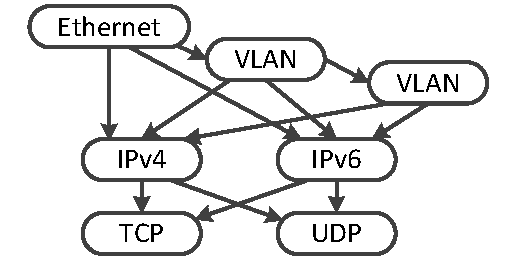
\includegraphics[width=\textwidth]{figs/parse-graph.pdf}
        		\caption{Parse Graph}
        		\label{parse-graph}
		\end{subfigure}
        \begin{subfigure}[t]{0.5\textwidth}
        		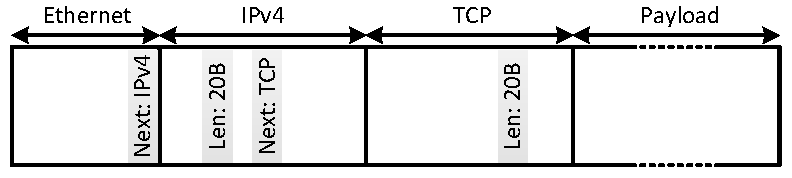
\includegraphics[width=\textwidth]{figs/packet.pdf}
        		\caption{TCP/IP Packet}
        		\label{packet}
		\end{subfigure}
\caption{An example parse graph commonly seen in enterprise networks, and a packet belonging to that parse graph. A parse graph can be used to represent the combinations of protocols that a packet processor may see in a certain application.}
\label{parse-graph-packet}
\end{figure}
%

Depending on the application, a packet processor must be able to process packets of a certain set of protocols.
These protocols vary depending on the type of packet and layer they represent on the OSI stack.
For example, Ethernet is one of the most common layer 2 protocols found in modern networks.
The protocol at each layer contains information regarding the type and location of the protocol found in the next higher layer (Figure~\ref{packet}).
The various different combinations of protocols that may be received in a single packet can be represented by a parsing graph~\cite{gibb2013design} (Figure~\ref{parse-graph}).

As network protocols are changed, added and replaced, a programmable packet processor must be able to be reconfigured to support different parsing graphs.
%OpenFlow-based processors use match tables to traverse these graphs.
The OpenFlow standard comes with specifications for architecting an SDN-compatible packet processor~\cite{opennet}.
The architecture is based on a cascade of match-action ``flow'' tables: memory holding all possible values of relevant packet header fields, and instructions for what action to be taken once matched.
Figure~\ref{openflow-pp} illustrates the high level design of this architecture.
The pipeline begins by matching fields whose locations in the packet header are known.
%When a field is matched at a table entry for a protocol at a certain OSI stack layer, the entry contains information regarding where to look in the next match table for the protocol of the next layer.
When a field is matched, the entry contains information regarding where to look in the next match table for the protocol of the next layer, as well as any other corresponding actions to be taken.
This model requires match tables to contain all possible combinations of header protocols and field values that the processor may face.
All of the tables in the pipeline are populated by the control plane, such that lookups in a Table \textit{j} can depend on information from any Table \textit{i} so long as \textit{i} $<$ \textit{j}.

%The OpenFlow standard comes with specifications for architecting an SDN-compatible packet processor~\cite{opennet}.
%The architecture is based on a cascade of match-action ``flow'' tables: memory holding all possible values of relevant packet header fields, and instructions for what action to be taken once matched.
%Figure~\ref{openflow-pp} illustrates the high level design of this architecture.
%The pipeline begins by matching fields whose locations in the packet header are known, and determining corresponding actions to take based on what values are matched.
%Information from these matches can then be used to determine the location of other packet header fields to perform matching in later stages of the pipeline.
%All of the tables in the pipeline are populated by the control plane, such that lookups in a Table \textit{j} can depend on information from any Table \textit{i} so long as \textit{i} $<$ \textit{j}.

There are two important limitations to this programmable packet processor design.
When built in an ASIC, the number of tables along with their width and depth are fixed upon chip fabrication.
Consequently, should a new protocol be created that requires fields that are larger than the table width, a number of entries that exceeds the table depth, or more pipeline stages than are available, then the packet processor can not be configured to support such a protocol.
Similarly, the action set available is also set upon fabrication.
Any new actions required by newly developed protocols could not be supported.

%
%
%


Recent work has revealed two possible ways to address these limitations.
Bosshart \textit{et al.} proposed building in additional programmability into an ASIC-based packet processor through the use of ternary content-addressable memory (TCAMs)~\cite{bosshart2013forwarding}.
Their design -- called RMT (Reconfigurable Match Tables) -- can be viewed as an upgrade to the OpenFlow model.
It involves mapping logical match (or flow) tables to physical ones by allowing a logical table to use resources from multiple pipeline stages.
This mapping process allows the width and depth of flow tables to be customized for specific sets of protocols.
Additionally, their design implements a reduced instruction set that, when used in combinations in a very-long instruction word, can execute a wider array of actions than OpenFlow.

The RMT design mitigates, but does not solve OpenFlow's limitations.
As the authors admit in the paper, their design is still restricted by the number of pipeline stages, table sizes, and action units made available to the chip upon fabrication.
These restrictions cannot be avoided when building a programmable packet processor from ASIC technology.
In contrast, Attig and Brebner have previously shown that a programmable packet parser can be built on an FPGA that supports 400 Gb/s bandwidth~\cite{attig2011400}.
Their design -- which they refer to as PP\footnote{Attig and Brebner use ``PP'' to refer to the language used to program their architecture. For simplicity, we shall use PP to refer to their design as a whole.} -- still uses a sequence of match tables, with each match stage determining the location of fields to be matched in the next stage.
Using an FPGA allows their design to be reconfigured in the field to support different table configurations and actions.

Our programmable packet processor design also leverages FPGA technology to avoid the limited flexibility of ASIC-based designs.
However, unlike the PP design, we elect to avoid using the recommended OpenFlow architecture, which was originally proposed to bring programmability to ASIC-based network infrastructures.
We instead embrace the full reconfigurability of the FPGA, creating a fully-programmable packet processor that is more efficient than the FPGA-based PP design and more flexible than the ASIC-based RMT design.

\figvs{1}{openflow-pp}{}{High-level overview of OpenFlow's programmable packet processor architecture~\cite{opennet}.}

%
%
%#############################################################
\vspace{\abovesectitle}
\section{The NoC Packet Processor}
\label{sec:design}
\vspace{\undersectitle}
%-0-0-0-0-0-0-0-0-0-0-0-0-0-0-0-0-0-0-0-0-0-0-0-0-0-0-0-0-0-0-
%
\subsection{Design Overview}
%
\comment{

1. Before performing any form of processing, a packet must be parsed in order to determine the header protocols
2. Various different combinations of protocols can be received --> this can be represented by a parsing graph
3. OpenFlow-based parsers have used match tables to traverse this graph: fields are matched with a certain entry in the table that contains information regarding which node to traverse to next
4. This model requires tables to contain all possible combinations of header protocols
5. Our key innovation replaces these tables with processing modules that are specific to one node in the parsing graph. Nodes that are small can be collapsed to form a larger node.
6. Nodes are interconnected using a full-crossbar
7. Full-crossbars are difficult to implement in FPGAs, as multiplexers do not synthesize well
8. Use the embedded NoC as the crossbar!!!

}
%

%

\figfull{2}{high-level-pp}{}{High level representation of module-based packet processor design. Packets are switched between processing modules corresponding to the protocols found in their headers.}

%\begin{figure}
%\centering
%%
%        \begin{subfigure}[t]{0.5\textwidth}
%        		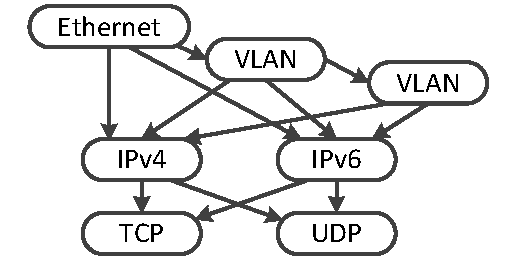
\includegraphics[width=\textwidth]{figs/parse-graph.pdf}
%        		\caption{Parse Graph}
%        		\label{parse-graph}
%		\end{subfigure}
%        \begin{subfigure}[t]{0.5\textwidth}
%        		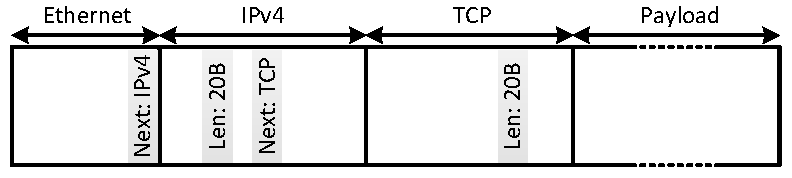
\includegraphics[width=\textwidth]{figs/packet.pdf}
%        		\caption{TCP/IP Packet}
%        		\label{packet}
%		\end{subfigure}
%\caption{An example parse graph commonly seen in enterprise networks, and a packet belonging to that parse graph. A parse graph can be used to represent the combinations of protocols that a packet processor may see in a certain application.}
%\label{parse-graph-packet}
%\end{figure}
%%
%
%Depending on the application, a packet processor must be able to process packets of a certain set of protocols.
%These protocols vary depending on the type of packet and layer they represent on the OSI stack.
%For example, Ethernet is one of the most common layer 2 protocols found in modern networks.
%The protocol at each layer contains information regarding the type and location of the protocol found in the next higher layer (Figure~\ref{packet}).
%The various different combinations of protocols that may be received in a single packet can be represented by a parsing graph~\cite{gibb2013design} (Figure~\ref{parse-graph}).
%
%As network protocols are changed, added and replaced, a programmable packet processor must be able to be reconfigured to support different parsing graphs.
%OpenFlow-based processors use match tables to traverse these graphs.
%When a field is matched at a table entry for a protocol at a certain OSI stack layer, the entry contains information regarding where to look in the next match table for the protocol of the next layer.
%This model requires match tables to contain all possible combinations of header protocols and field values that the processor may face.

%
%\begin{figure}[t] \centering
%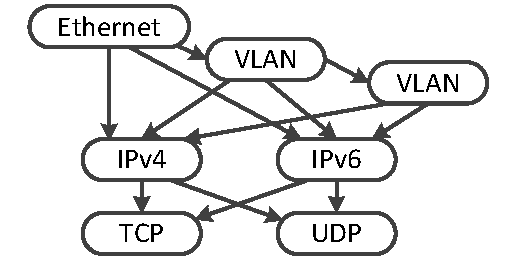
\includegraphics[width=0.35\textwidth]{figs/parse-graph.pdf}
%\caption{An example parse graph commonly seen in enterprise networks. A parse graph can be used to represent the combinations of protocols that a packet processor may see in a certain application.}
%\label{parse-graph}
%\vspace{0cm}
%\end{figure}
%

Instead of match tables that each support a set of protocols, our design implements multiple processing modules, with each module dedicated to processing a single parsing graph node's protocol (Figure~\ref{parse-graph}).
Packets are sent to the modules corresponding to the protocols found in their headers.
Each processing module determines what actions to take for its protocol, and the type and location of the protocol processing module for the packet's next OSI layer.
%For example, consider a packet consisting of Ethernet, IPv4, and TCP headers (as in Figure~\ref{packet}).
%Such a packet would first be forwarded to an Ethernet processing module, where it would be discovered that the protocol of the next header is IPv4.
%Once Ethernet processing is complete, the packet would then be sent to an IPv4 processing module, and finally to a TCP processing module.
%Another packet containing Ethernet, IPv6, and TCP headers would follow nearly the same path, except instead of being sent to an IPv4 processing module, it would be sent to one for IPv6.
Figure~\ref{high-level-pp} depicts a general representation of this packet processor design.

The FPGA reconfigurable fabric is used to implement the processing modules.
The flexibility of the fabric allows for the modules to be fully customized and later updated, as existing protocols are enhanced and new protocols are added.
It is by updating the modules that processing rule updates are made.
For example, in order to modify the supported parse graph, each module's routing decision logic is updated to match the new set of edges connecting its corresponding node in the graph.
Module updates are made by reconfiguring (or partially reconfiguring, see Section~\ref{sec:reconfig}) the FPGA.

%As in any packet processor, the processing modules perform some set of actions when packet fields are matched.
%However, since each processing module is dedicated to a single node in the parsing graph, its matches and actions are tied solely to what is relevant to that node.
%It is by updating the modules that processing rule updates are made.
%Field matches, actions, routing decision logic 
%In order to modify the supported parse graph, each module's routing decision logic is updated to match the new set of edges connecting its corresponding node in the graph.
%Field matches and routing decisions at a particular protocol node can be stored in tables at the module.
%These tables only need to contain entries relevant to actions that can take place for that protocol, unlike the OpenFlow flow tables, which must have entries for all possible field matches at that stage.
%In effect, a flow table is broken up and spread across several processing modules.
%The module tables' widths and depths, as well as the modules actions, can be customized to fit only the module's protocol.
%We argue that having these ``fine-grained'' tables that are specifically customized for a protocol will allow for a more efficient design than OpenFlow's ``coarse-grained'' flow tables.
%For example, an OpenFlow flow table that is expecting either IPv4 and IPv6 packets must be made wide enough to match the 128-bit address fields of IPv6, despite the fact that IPv4 addresses are only 32 bits.
%If there are many more IPv4 addresses to be matched, then the table would also have to be deep enough to hold all the address entries.
%In contrast, our design would have an IPv4 module with a match table that is deep enough to hold all the entries, but only need to be wide enough to hold the 32-bit addresses.
%Similarly, the IPv6 module table could be made shallow and wide.


Interconnecting the processing modules is a challenging problem on current FPGA devices.
Multiplexers, which are necessary for the full crossbars in Figure~\ref{high-level-pp}, are synthesized poorly on the FPGA's fabric, often consuming relatively high chip area and running considerably slower than they would if built in ASIC technology.
A full crossbar that is wide enough to support the very high bandwidth of data entering modern packet processors would be very difficult, if not impossible, to efficiently synthesize in the FPGA fabric.

%Besides module duplication, the NoC-PP design also allows for the easy addition and/or removal of protocols as needed.
%Say a new protocol has been developed and must be supported by the packet processor.
%A processing module for this protocol can then be designed and added to the NoC-PP by connecting it to any of the routers in the NoC, with little other modification to the rest of the design.
%Similarly, if a protocol no longer needs to be supported, then its processing modules can simply be removed from the design.


%
\subsection{The NoC-Crossbar}
%
\comment{

1. Use the embedded NoC as the crossbar!!!
2. NoC flow control
3. NoC characteristics (radix, topology, link width, frequency, BW)
4. How to use NoC as crossbar
5. How to connect more than just 16 modules (arbiter design and block diagram)

}
%

To address this problem, we draw inspiration from previous work that used an embedded NoC in an FPGA as a crossbar for an Ethernet switch~\cite{bitar2014efficient,abdelfattah2015take}.
This NoC -- described in Section~\ref{sec:noc-fpga} -- can function as the full crossbar in our packet processor design.
Not only is it already designed to transfer packets across the FPGA, it also includes a built-in flow control mechanism that can handle scenarios of adversarial traffic, such as prolonged bursts of packets.
For example, if a certain processing module is busy and cannot accept packets from the NoC, the NoC will hold packets destined for that module in a buffer at the connecting router.
Should that buffer become full, packets will then be buffered at downstream NoC routers.
If the NoC cannot accept packets at one of its routers due to a buffer being full, then it can also send a backpressure signal to the modules connected to that router.

%\hl{consider removing this text in favour of embedded NoC section}
%The NoC used in our design is a 16-node mesh with 150b-wide links and capable of running at 1.2 GHz in 28-nm process technology (the same process used for Stratix-V devices).
With a capacity of 180 Gb/s at each of its links, the NoC can transport high bandwidth data throughout the FPGA, to and from processing modules in our design.
Processing modules are connected to NoC routers, as illustrated in Figure~\ref{noc-parser-general}, with the NoC's FabricPort used to bridge the frequency of the processing modules and the frequency of the NoC (see Section~\ref{sec:noc-fpga}).
%In effect, this design uses the embedded NoC to replace the full crossbars in Figure~\ref{high-level-pp}.
Moreover, we can combine multiple modules at a single router node using the FPGA's soft logic for arbitration.
For the remainder of the paper, we shall refer to this NoC packet processor as ``NoC-PP''.

%In order to not be limited to a maximum of 16 processing modules, we created arbitration logic to connect multiple modules to a single NoC router (Figure~\ref{arbiter}).
%To maximize independence between each module connected to the router, FIFO queues were added between each module and the arbitration logic.
%This allows for each module to independently send and receive backpressure to and from the NoC.
%The queue depth depends on the number of modules connected and the desired degree of independence between modules.

%
\figvs{1}{noc-parser-general}{}{The ``NoC-PP'' architecture: the embedded NoC serves as the crossbar for the module-based packet processor design. NoC routers and links are ``hard'', i.e. embedded in the chip, while the processing modules and arbitration logic are synthesized from the FPGA ``soft'' fabric.}
%

%
%\figvs{1}{arbiter}{}{Arbitration logic for connecting multiple processing modules to a single NoC router.}
%

%
\subsection{Inter-Module Information Passing}
%
\comment{

1. Header data beat added to allow vector of parsed fields to be created
2. Header data beat also holds offset to tell processing module where in the header the protocol is located

}

Thus far, we have described a mechanism for processing protocols with modules that are independent of one another.
However, packet processing requires at least some information to be passed from one protocol to another.
As a bare minimum, information regarding where the next protocol's header is located in the packet is determined in the previous protocol header and therefore must be passed to the next protocol's processing module (see Figure~\ref{packet}).
There are many other possible scenarios where information from a lower-level protocol may be used later in the processing stages.
For example, in packet classification, a classification decision may be made after a combination of fields are parsed from each of the packet's headers.

To provide a mechanism for information-passing between processing modules, the NoC-PP design adds a blank header flit to every packet upon entering the processor.
This header flit can hold any combination of parsed fields from the packet as it proceeds through the processor.
Data stored in the header flit are maintained across processing modules until they are overwritten.
For example, our design stores a 7-bit ``data offset'' field in this header flit that is updated by every processing module.
This field tells the next processing module where its header is located in the packet.
The header flit is removed just before the packet exits the processor.

%
\subsection{Design Example: Eth-IPv4/IPv6-TCP}
\label{sec:design-example}
%
\comment{

1. For this paper, we design and evaluate for a specific and common application
--> allows for comparison to previous work (Brebner)
2. Describe architecture of processing modules
3. Describe processing features of each processing module
4. Describe data path width and frequency
>> Describe process of packets how they traverse the processor 
5. Show how duplication of modules allows for the support of higher bandwidth
6. Show how using both directions of the NoC can double supported BW
7. Highlight customizability of this design
- new protocols can be added
- more modules can be added to support more throughput
- some protocols don't have to be duplicated as much if we know that there traffic is low (see evaluation section)

}
%

In order to evaluate this design, we implemented a packet processor that supports processing of several common network protocols: Ethernet, VLAN, IPv4, IPv6, and TCP.
Table~\ref{tbl:proc} lists the features implemented in each of the protocol processing modules.
%Each of the processing modules follows a similar architecture.
%Packets arriving at the modules are sent through pipeline registers, while module-specific logic performs the processing functions in parallel.
Each packet going through the processor will visit a processing module for each protocol found in its header.
For example, consider an Ethernet/IPv4/TCP packet.
The packet is first brought onto the chip through the FPGA's transceivers, which perform clock recovery and serial to parallel data conversion.
It is then transported to the embedded NoC through the FPGA's soft interconnect, where the FabricPort (Section~\ref{sec:noc-fpga}) performs clock conversion to bring the data from the slower FPGA fabric to the fast NoC.
The NoC's links and routers steer the packet to a router connected to an Ethernet processing module, where the FabricPort again performs clock conversion to bring the packet back to the FPGA fabric.
Once Ethernet processing is complete and the next layer protocol is determined, the packet is then brought back to the NoC to be sent to an IPv4 processing module, and finally a TCP processing module, before being sent back out through the FPGA's transceiver.

%The number of pipeline registers implemented is equal to the number of processing cycles required before the packet can be sent.

%
%
\begin{table}[!t]
\centering
\begin{small}
    \caption{Functions implemented in each protocol processing module in our NoC-PP design.}
    \label{tbl:proc}
    \begin{tabular}{ll}
    \toprule
    \textbf{Protocol} & \textbf{Implemented Processing Functions} \\
    \textbf{Module} &  \\
    \midrule
	Ethernet/VLAN & 1. Parse MAC source and destination   \\ 
	              & 2. Maintain a MAC table with address-port \\
	              &    mappings \\
	              & 3. Extract priority code identifier (PCP) in \\
	              &    VLAN header \\
	              & 4. Determine layer 3 protocol from Ethertype \\
	\midrule
	IPv4          & 1. Compute checksum and drop packet if  \\
	              &    results in error    \\
	              & 2. Decrement time to live (TTL) and drop \\
	              &    packet if zero reached\\
	              & 3. Determine total length of header \\
	              & 4. Parse source and destination IP addresses \\
	              & 5. Determine layer 4 protocol \\
	\midrule
    IPv6          & 1. Decrement hop limit and drop packet if \\
    			  &    zero reached   \\
    			  & 2. Parse source and destination IP addresses \\
    			  & 3. Determine layer 4 protocol \\
    \midrule
    TCP           & 1. Parse source and destination ports    \\
    			  & 2. When receiving a request to establish a \\
    			  &    connection, generate and send a reply ACK \\
    			  &    message over TCP/IP \\
    \bottomrule
    \end{tabular}
\end{small}
\end{table}
%
%

%\figvs{1}{processing-module}{}{General architecture of processing modules in NoC-PP.}

%
\begin{figure*}
\centering
%
        \begin{subfigure}[t]{0.45\textwidth}
        		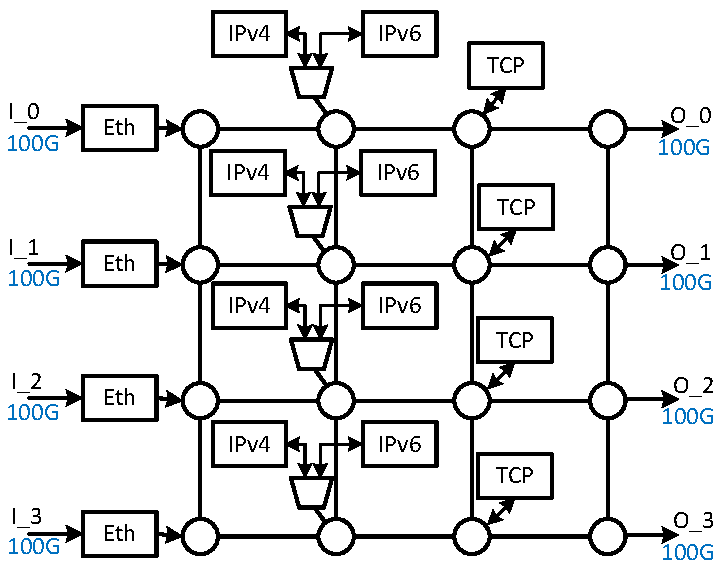
\includegraphics[width=\textwidth]{figs/noc-pp-uni.pdf}
        		\caption{400G}
        		\label{400g}
		\end{subfigure}
        \begin{subfigure}[t]{0.45\textwidth}
        		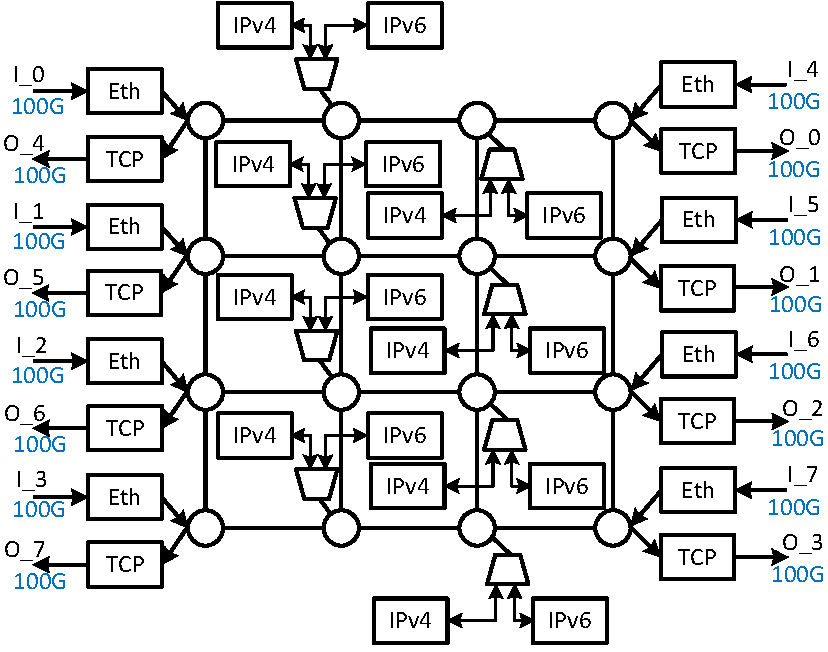
\includegraphics[width=\textwidth]{figs/noc-pp-bi.pdf}
        		\caption{800G}
        		\label{800g}
		\end{subfigure}
\caption{The NoC PP design for an Ethernet/VLAN/IPv4/IPv6/TCP packet processor (Eth=Ethernet+VLAN). Processing modules run at 100G, and are instantiated four times to support 400G processing, or eight times to support 800G processing.}
\label{noc-pp}
\end{figure*}
%

The processing modules are designed with a data path width of 512 bits running at 200 MHz, providing an overall processing throughput of 100 Gb/s.
There are two possible ways for this design to support a higher network bandwidth: increase the supported throughput of the individual processing modules or instantiate multiple instances of the processing module throughout the NoC.
In our design, we duplicate the 100G processing modules to provide higher overall processing bandwidths, such as 400G and 800G (Figure~\ref{noc-pp}).
This ability to duplicate individual processing modules provides a key form of design flexibility not found in previously proposed packet processor designs.
If a designer is aware of the expected frequencies of traffic of each of the different protocols, then he/she can duplicate the different processing modules to the appropriate degree.
For example, if IPv4 packets are currently much more frequent compared to IPv6 packets, then the design could instantiate more IPv4 processing modules than IPv6.
This design flexibility is explored in Section~\ref{sec:flex}.

Besides module duplication, the NoC-PP design also allows for the easy addition and/or removal of protocols, thanks to the logical and physical decoupling of processing modules by the NoC.
Say a new protocol has been developed and must be supported by the packet processor.
A processing module for this protocol can then be designed and added to the NoC-PP by connecting it to any of the routers in the NoC, with little other modification to the rest of the design.
Similarly, if a protocol no longer needs to be supported, then its processing modules can simply be removed from the design.


%
%
%#############################################################
\vspace{\abovesectitle}
\section{Evaluation}
\label{sec:eval}
\vspace{\undersectitle}
%-0-0-0-0-0-0-0-0-0-0-0-0-0-0-0-0-0-0-0-0-0-0-0-0-0-0-0-0-0-0-
%
\subsection{Simulation and Synthesis Setup}
\label{sec:setup}

We use \texttt{\textbf{RTL2Booksim}}~\cite{fpl15demo} to connect the packet processing modules to the embedded NoC, and perform a cycle-accurate simulation in ModelSim. 
This allows us to gather our performance data in cycle counts; however, we also need to find the operating frequency of our packet processing modules to be able to quantify the overall performance of NoC-PP.
Furthermore, we want to realistically model any physical design consequences of connecting these packet processing modules to embedded routers (such as interconnection choke-points or possible frequency degradation).
To do so, we emulate the existence of routers in an Altera FPGA (Stratix V 5SGSED8K1F40C2) by creating 16 design partitions -- one for each router -- that have the same size, location and interconnection flexibility as an embedded router.
We then connect our packet processing modules to them the same way they are connected in NoC-PP and compile the design in Quartus II v14.0 to collect the area and frequency results presented in this section.


%
\subsection{Design Efficiency}
\vspace{-0.1cm}
%
\comment{

1. Want to compare to Brebner's 400G FPGA packet parser to highlight how we take better advantage of the FPGA platform
2. Quote Horowitz paper's claimed limitations of FPGAs
3. We first remove the processing functions of our design to stick only to parsing in order to do a fair comparison --> stick to the fields listed as parsed in the Brebner paper
4. Also synthesize the full processor design
5. We synthesize on a Stratix V-GS
6. Convert Brebner's Virtex 7-870HT numbers to Stratix V-GS
7. Show how our design is significantly more efficient, but the degree to which it is better diminishes as the design grows
8. Not surprising, since our design is based on a "only use what you need" principle, whereas the PP design requires an established pipeline of tables to be present regardless of the complexity of the parser

}
%

The PP packet processor design maintains OpenFlow's cascade of flow tables architecture, despite using an FPGA.
OpenFlow's flow table design was created to add programmability to ASIC-based network infrastructures.
Bosshart \textit{et al.} argue that FPGA's are poorly suited for such an architecture, as they offer far lower total memory capacity compared to their RMT chip design~\citep{bosshart2013forwarding}.
Using this argument, the authors rule out FPGA technology for programmable packet processors.
We argue that an FPGA can overcome its memory limitations by using our module-based NoC-PP architecture that significantly reduces the design's reliance on memory.

To demonstrate this, we measure the hardware cost and performance of the NoC-PP design and compare it to Attig and Brebner's PP design.
PP, however, only provides packet parsing functionality.
It extracts fields from the packets but does not perform any form of action after the extraction, besides determining where the next header is located.
Consequently, we also synthesized a modified version of the NoC-PP design that only contains parsing functionality, thus providing a fair comparison.
We compare to two versions of the PP design: (1) the smallest, ``JustEth'', which only performs parsing on the Ethernet header, and (2) one of their biggest, ``TcpIp4andIp6'', which performs parsing on Ethernet, IPv4, IPv6 and TCP~\cite{attig2011400}.

Table~\ref{tbl:results} contains hardware cost and performance results of the NoC-PP and the PP designs.
Hardware cost is measured using resource utilization as a percentage of an Altera Stratix V-GS FPGA.
Attig and Brebner's experimental results, originally presented as a percentage of a Xilinx Virtex-7 870HT FPGA, are converted to equivalent Stratix V-GS numbers.
To perform this conversion, we use equivalent logic element/logic cell counts on each device, which we have found to accurately reflect the logic capacity for both vendors across a large number of designs.
The resource utilization results for the NoC-PP design also include the resources consumed by RAM blocks and the embedded NoC~\cite{abdelfattah2015take}.
The table also contains results for the full packet processor described in Section~\ref{sec:design-example} at 400G and 800G, referred to as ``TcpIp4Ip6-Processor'' (illustrated in Figure~\ref{noc-pp}).
Figure~\ref{800G-floorplan} shows the floorplan of the FPGA with the synthesized 800G TcpIp4Ip6-Processor design.


\begin{table}[t]
\center
\caption{Comparison of the NoC-PP and PP architectures}
\begin{tabular}{lllll}
\toprule
 \textbf{Application} & \textbf{Architecture} & \textbf{Resource} & \textbf{Latency} & \textbf{Throughput} \\
 & & \textbf{Utilization} & \textbf{(ns)} & \textbf{(Gb/s)} \\
 & & \textbf{(\% FPGA)} & & \\
\midrule
\multirow{2}{*}{JustEth} &  NoC-PP  & 3.6\%  & 79 & 410 \\
                         &  \cellcolor{gray!25}PP~\cite{attig2011400}      & \cellcolor{gray!25}11.6\% & \cellcolor{gray!25}293 & \cellcolor{gray!25}343 \\
\midrule
\multirow{2}{*}{TcpIp4Ip6} &  NoC-PP  & 9.4\%  & 200 & 410 \\
                           &  \cellcolor{gray!25}PP~\cite{attig2011400}      & \cellcolor{gray!25}15.6\% & \cellcolor{gray!25}309 & \cellcolor{gray!25}325 \\
\midrule
TcpIp4Ip6        &  \multirow{3}{*}{NoC-PP}  & \multirow{3}{*}{14.4\%}  & \multirow{3}{*}{230} & \multirow{3}{*}{410} \\
-Processor & & & & \\
(400G) & & & & \\
\midrule
TcpIp4Ip6        &  \multirow{3}{*}{NoC-PP}  & \multirow{3}{*}{25.8\%}  & \multirow{3}{*}{232} & \multirow{3}{*}{819} \\
-Processor & & & & \\
(800G) & & & & \\
\bottomrule
\end{tabular}
\label{tbl:results}
\end{table}

\figvs{0.9}{800G-floorplan}{}{Floorplan of the 800G NoC-PP ``TcpIp4Ip6-Processor'' design synthesized on a Stratix-V FPGA. The orange rectangles indicate the reserved partitions used to emulate the embedded NoC. The black regions are unused area on the chip. Note that the coloured logic blocks may be only partially filled.}

%\begin{figure}[!t]
%\centering
%\includegraphics[width=#1\columnwidth,keepaspectratio,#3]{figs/#2}
%\caption{#4}
%\label{#2}
%\end{figure}

Overall, the NoC-PP proves to be more resource efficient and achieves better performance compared to the PP architecture.
Interestingly, the degree to which NoC-PP is more resource efficient varies depending on the application.
For the smaller application (JustEth), the NoC-PP design is 3.2$\times$ more efficient, whereas for the larger application (TcpIp4Ip6), it is 1.7$\times$ more efficient.
This can be explained by the ``only use what you need'' design policy of NoC-PP: processing modules are dedicated to a single protocol and only included in the design if the processor must support that protocol.
In contrast, the PP design is based on a pipeline of match tables that must be included no matter how few protocols need to be supported.
The match table overhead is the main reason why the PP design is significantly less efficient compared to NoC-PP.
Furthermore, NoC-PP also reduces latency by 3.7$\times$ and 1.5$\times$ compared to PP for JustEth and TcpIp4Ip6, respectively.
Table~\ref{tbl:results} also shows that our full-featured packet processor is still more efficient than the more basic packet parser presented in prior work.
Lastly, it is worth noting that the 800G design achieves a throughput greater than any previously reported packet processor built from an FPGA.
Thus, the module-based NoC-PP architecture provides significant advantages for FPGA packet processors.




%
\vspace{-0.1cm}
\subsection{Design Flexibility}
\label{sec:flex}
%
\comment{

--> Talk about how, to support future network bandwidths, the NoC can scale by widening the links

1. Benefit of the NoC-PP modular design is it allows for the easy addition or removal of protocol processing modules
2. This can be used to introduce new protocols or duplicate existing modules to process certain protocols at a higher bandwidth (discussed previously)
3. The 400G use-case of the NoC-PP consists of four duplicates of each protocol's processing module
4. Duplication of a certain protocol can be reduced in order to free up room for other processing modules
5. We would like to explore the impact of removing processing module on performance

}
%

%
\begin{figure*}
\centering
%
        \begin{subfigure}[t]{0.45\textwidth}
        		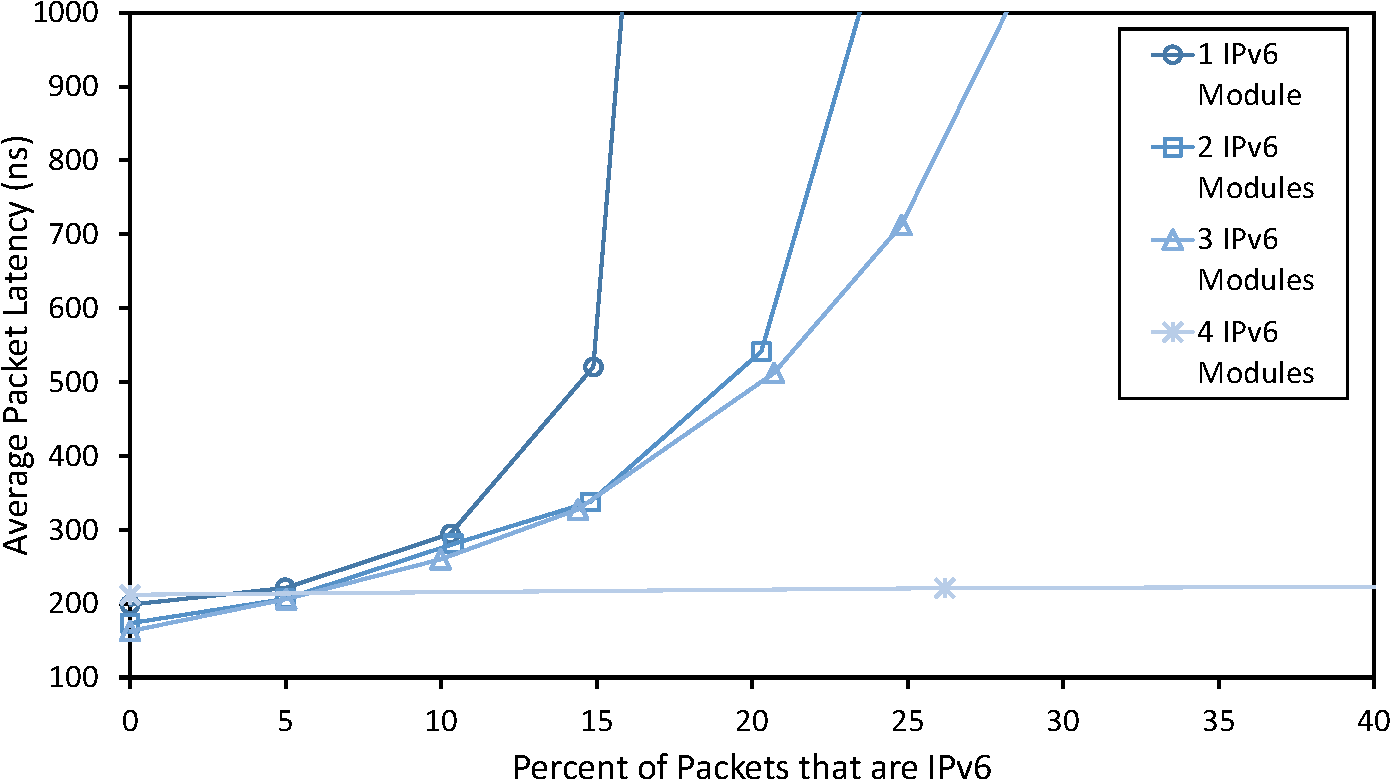
\includegraphics[width=\textwidth]{figs/latency-modules-plot.pdf}
        		\caption{NoC Router Buffer Depth = 10 flits}
        		\label{latency10}
		\end{subfigure}
        \begin{subfigure}[t]{0.45\textwidth}
        		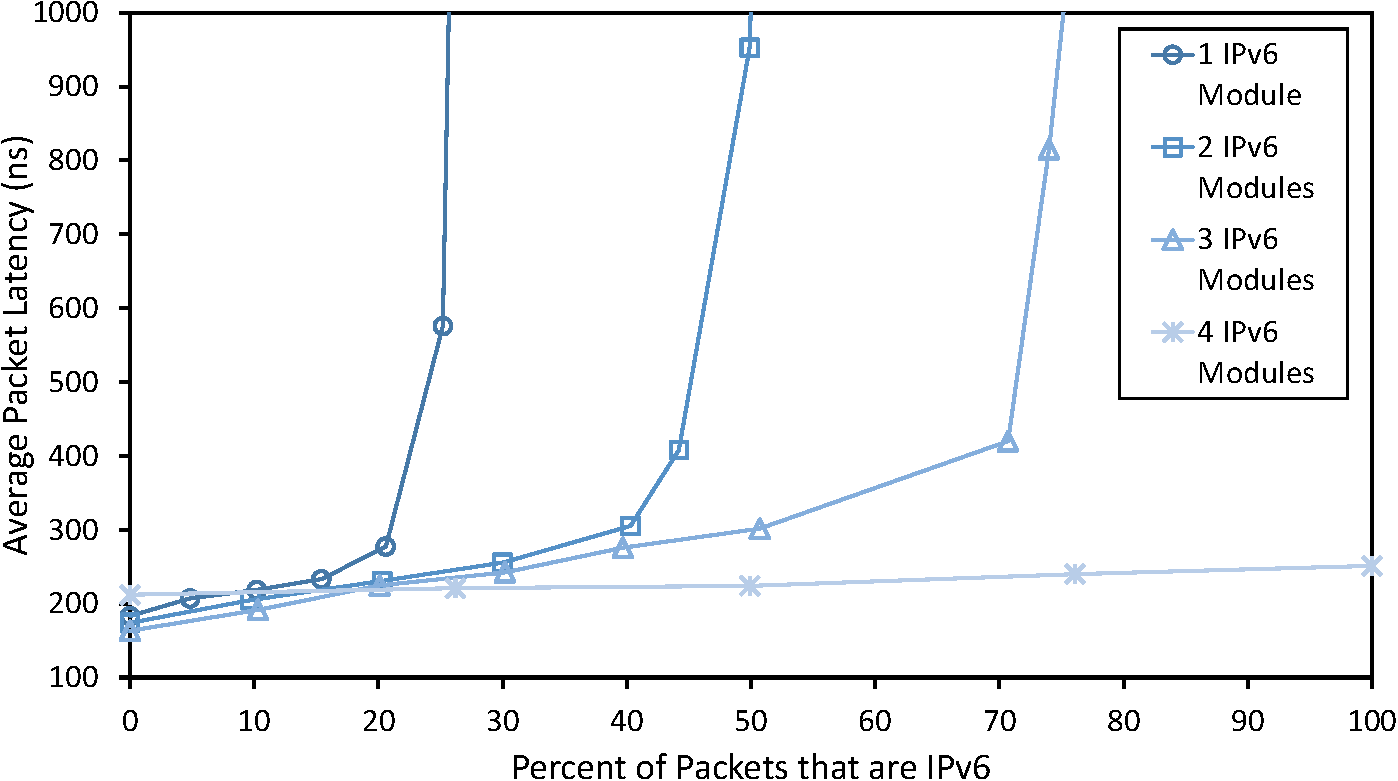
\includegraphics[width=\textwidth]{figs/latency-modules-plot2.pdf}
        		\caption{NoC Router Buffer Depth = 64 flits}
        		\label{latency64}
		\end{subfigure}
\caption{Average packet latency through the NoC-PP design as a function of percentage of total traffic using IPv6, for four different degrees of IPv6 module duplication. Four IPv6 modules (each running at 100G) is sufficient to fully support any rate of IPv6 traffic running at 400G.}
\label{latency-modules}
\end{figure*}
%

%
\begin{figure*}
\centering
%
        \begin{subfigure}[t]{0.4\textwidth}
        		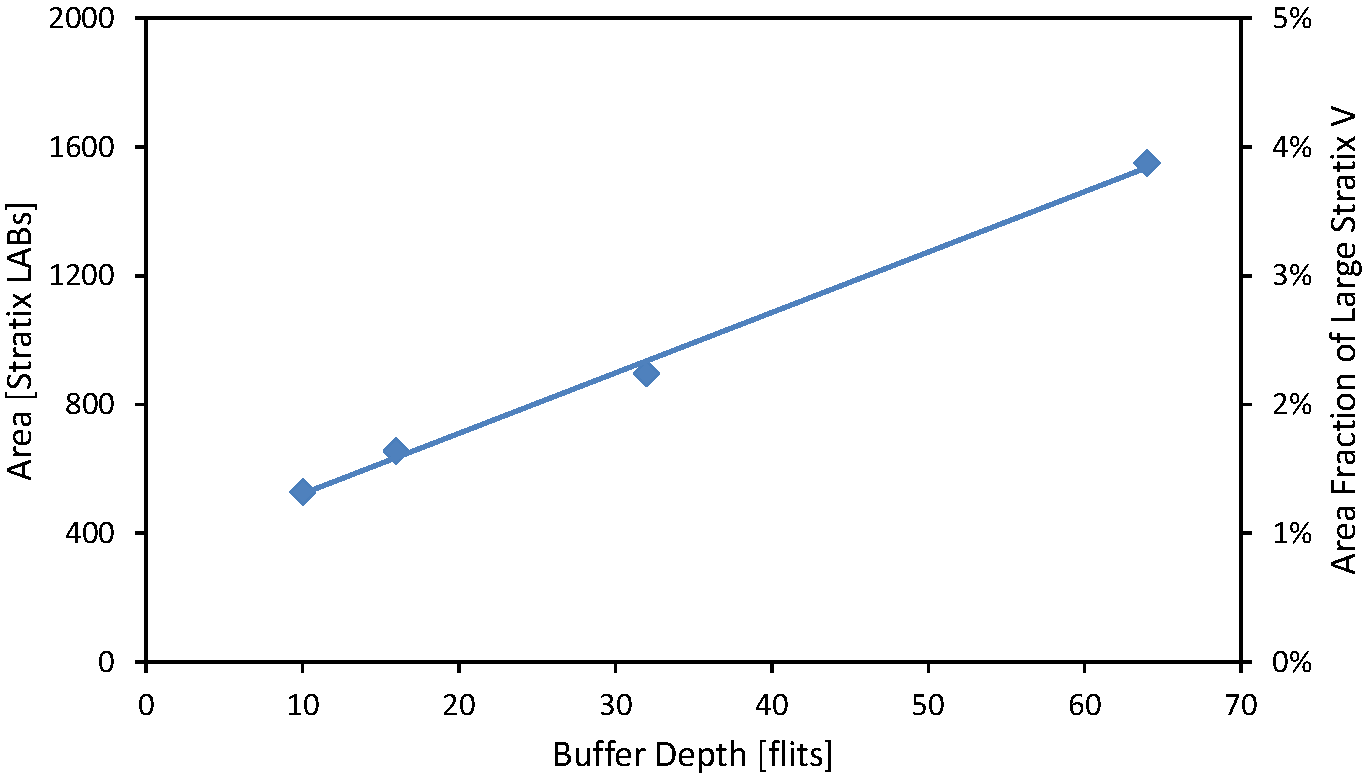
\includegraphics[width=\textwidth]{figs/buffer-depth.pdf}
        		\caption{Embedded NoC Area Scaling with Buffer Depth}
        		\label{buffer-depth}
		\end{subfigure}
        \begin{subfigure}[t]{0.4\textwidth}
        		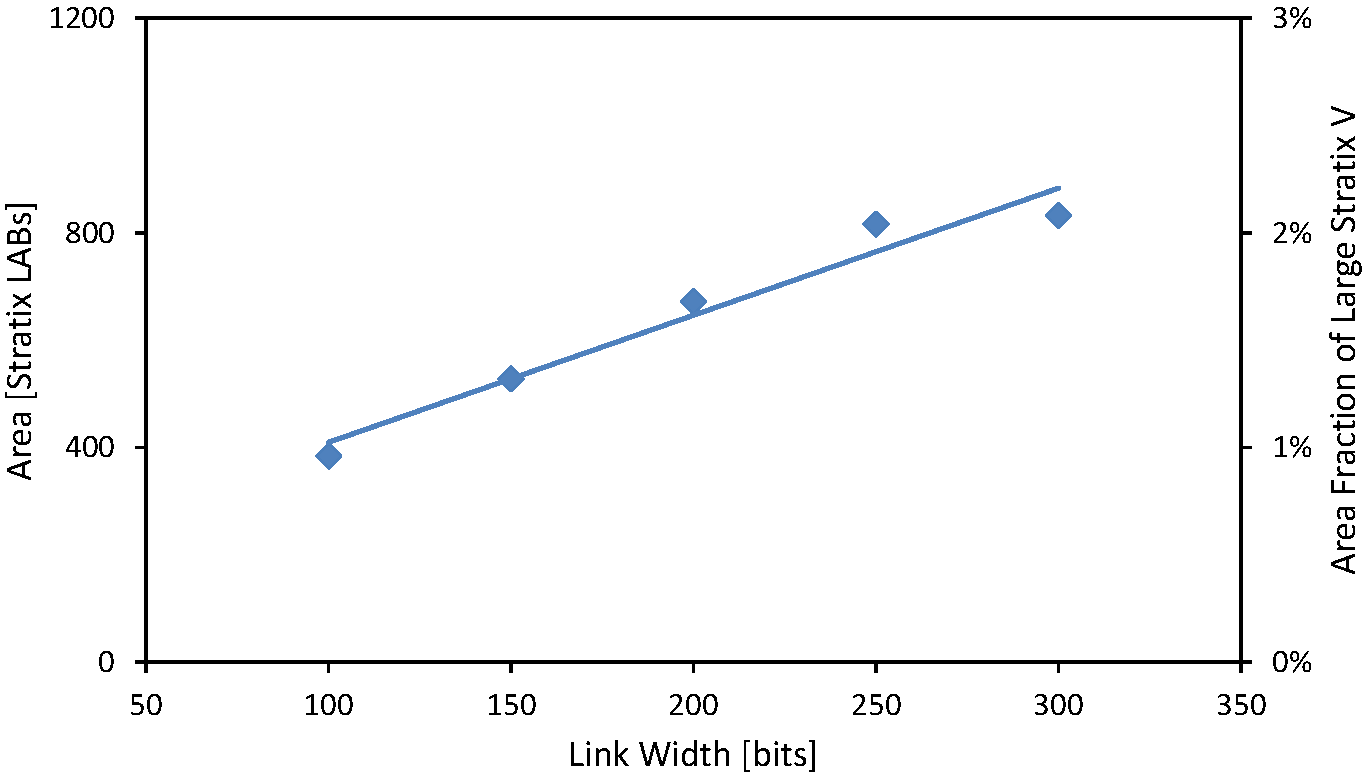
\includegraphics[width=\textwidth]{figs/link-width.pdf}
        		\caption{Embedded NoC Area Scaling with Link Width}
        		\label{link-width}
		\end{subfigure}
\caption{Embedded NoC chip area, measured in equivalent Stratix LABs and fraction of a Stratix V-GS, scaling with buffer depth and link width~\cite{noc-designer}. Figure~\ref{buffer-depth} plots buffer depth with a fixed link width of 150 bits, while Figure~\ref{link-width} plots link width with a fixed buffer depth of 10 flits.}
\label{noc-area}
\end{figure*}
%

The highly modular design of NoC-PP allows for the easy addition and removal of protocol processing modules.
This flexibility can be used to introduce new network protocols, modify protocol processing modules, and duplicate existing protocol modules in order to support higher bandwidths.
The TcpIp4Ip6-Processor design example duplicates each 100G processing module four and eight times in order to fully support 400G and 800G processing, respectively, for each protocol.
Depending on the application, full duplication of each processing module may not be necessary.
It is possible, for example, that a low percentage of the traffic seen by the packet processor uses IPv6\footnote{As of July 2015, Google measures that only $\sim$7\% of accesses to their website are through IPv6~\cite{google_ipv6}.}.
The designer therefore has the flexibility to reduce the number of IPv6 processing modules in order to free up chip area for other modules.

To assess the impact of module duplication on performance, we use \textbf{\texttt{RTL2Booksim}} to simulate the design with varied degrees of duplication of the IPv6 processing module, swept across percentage of the total traffic that is IPv6.
A bursty, 400G traffic pattern is used to emulate real Internet traffic, with packet payload size set to be 512 bytes.
The design is first simulated using a NoC consisting of the same parameters (link width, mesh radix, router buffer depth) as those chosen in previous work~\cite{abdelfattah2015take}.
Figure~\ref{latency10} illustrates the results.
The ``knee'' in each curve indicates the maximum percentage of IPv6 that can be supported at 400G; after this point, the NoC saturates, causing the source to be frequently backpressured.

%\figvs{1}{latency-modules-plot}{}{Average packet latency through the NoC-PP design as a function of percentage of total traffic using IPv6, for four different degrees of IPv6 module duplication. Four IPv6 modules (each running at 100G) is sufficient to fully support any rate of IPv6 traffic running at 400G.}

Originally, it was expected that the design would be able to support up to a fraction of IPv6 packets equal to the number of IPv6 modules implemented divided by four, given it takes four modules to fully support a 100\% IPv6 packet rate (i.e. 25\% for one IPv6 module, 50\% for two, etc.).
However, we see in Figure~\ref{latency10} that the NoC saturates at a much earlier point in each curve.
This can be attributed to the fact that the NoC is not an entirely non-blocking crossbar; packets compete for resources and when one does not receive access to its desired link, it must be held in buffers within the NoC.
In this case, the NoC routers have buffers that can hold 10 NoC flits~\cite{abdelfattah2015take}, while each injected packet forms 40 NoC flits.
Thus, when one packet is waiting for a NoC link to become free, it must be stored in four buffers, consequently congesting four downstream routers.
%When there is more of a mixture of IPv6 along with IPv4 packets, there is more switching in the NoC, as some packets are sorted to either an IPv6 or an IPv4 module.
%With more switching comes more conflicting resource requests, causing congestion to occur.
In the case when four IPv6 modules are implemented, each injection point has its own IPv6 module for its IPv6 packets.
Thus, there is no competition for resources in the NoC.
As soon as there is a mismatch in number of injection points and number of IPv6 modules, packets may compete for resources when two are sent to one IPv6 module at the same time.

One way to mitigate this congestion is to offload the packet payload to external memory until the packet is ready to be sent out, thereby reducing the amount of NoC buffer space consumed by a packet during processing.
This is briefly discussed in Section~\ref{sec:ddr}.
Another method is to increase the buffer depth in the NoC routers.
The impact of buffer size on NoC performance has been studied extensively in previous work~\cite{coenen2006buffer}.
In our application, if a router's buffer could hold an entire packet, rather than just a quarter, it would prevent downstream routers from becoming congested as well.
We test this theory by adjusting the simulated NoC buffer size to 64 flits, rather than 10.
As can be seen in Figure~\ref{latency64}, increasing the buffer size mitigates the NoC's blocking nature, allowing it to saturate according to the availability of IPv6 processing bandwidth in the design.

\vspace{-0.1cm}

The impact of increasing the buffer size of the NoC on its hardware cost is illustrated in Figure~\ref{noc-area}.
Increasing NoC buffer size allows the NoC-crossbar to provide more switching capability for larger packets at a moderate hardware cost.
Figure~\ref{noc-area} also shows the cost of increasing the NoC's inter-router links, which can be used to scale the NoC-crossbar to serve more network bandwidth.
Both of these scaling techniques require architectural changes to an embedded NoC.
Thus, it is crucial that a manufacturer of a NoC-enhanced FPGA appropriately provisions the NoC to serve potential applications.
%We hope our research in this paper and in previous work serves useful for this purpose.
By looking at important FPGA networking applications such as switching~\cite{bitar2014efficient,abdelfattah2015take} and packet processing, we hope to better guide the architectural choices of an embedded NoC.

\vspace{-0.1cm}

Overall, we see that the flexibility that NoC-PP provides to support reprogrammability for network evolution surpasses that of any conceivable ASIC-based packet processor.
NoC-PP is only limited by the amount of resources available on the entire FPGA.
Unlike the RMT design, NoC-PP is not limited by the table sizes and action set established upon chip fabrication.
New actions and match field values can be reprogrammed into new or existing processing modules at any time.
Modules can be modified, replaced and even duplicated by reconfiguring the FPGA fabric.
Not only does NoC-PP manage to exceed the flexibility of the ASIC-based RMT, but it also matches and surpasses RMT's supported bandwidth of 640G.




\vspace{-1mm}
%
%
%\subsection{Design Scalibility}
%\label{sec:scale}
%\input{scalability}
%
%#############################################################
%\vspace{\abovesectitle}
\section{Design Enhancements}
\label{sec:disc}
\vspace{-1mm}
%\vspace{\undersectitle}
%-0-0-0-0-0-0-0-0-0-0-0-0-0-0-0-0-0-0-0-0-0-0-0-0-0-0-0-0-0-0-
%
\subsection{Virtual Channel Priority Scheme}
\vspace{-1mm}
%
\comment{

1. The selected embedded NoC contains two Virtual Channels, as previous work has shown it improves performance (?) by 30\%
2. Virtual channels are...
3. With two virtual channels, data flowing through the packet processor can be sorted into two groups of traffic
4. This can be useful for establishing a packet priority scheme
5. Packet priority is prevalent in many different modern network protocols, including VLAN and TCP
6. Priority packets can have their own reserved VC, while all other traffic is routed through the other VC

}
%


Virtual Channels (VC) in a NoC are separate FIFO buffers located at every router port.
They allow packets arriving at or being sent along a common physical link to be stored in separate buffers.
The embedded NoC used in our design employs two VCs, as previous work has shown that NoC congestion is reduced by $\sim$30\% when a second VC is used~\cite{fpl}.
With two VCs, data flowing through the packet processor can be sorted into two groups of traffic.
This can be especially useful for establishing a packet priority scheme.
Packet priority is prevalent in many different modern network protocols, including VLAN and TCP.
In NoC-PP, one VC can be reserved for packets given priority based on the contents of their headers, while all other traffic is routed along the other VC.
Thus, priority packets can bypass non-priority packets when the NoC is congested, thereby giving priority packets a faster path through the design.



%\vspace{-1mm}
%
\subsection{Partial Reconfiguration}
\label{sec:reconfig}
\vspace{-0.1cm}
%
\comment{

1. Benefit of OpenFlow's flow table architecture: being able to reconfigure on the fly
2. Performing full FPGA reconfiguration cannot be done on the fly
3. Partial reconfiguration could solve this, but has yet to be proven to be feasible
4. The NoC is more amenable to partial reconfiguration, as modules are decoupled (don't have to have same clock either)
5. Partial reconfiguration of individual processing modules has the potential to be done on the fly
6. Left for future work

}
%

A key advantage to OpenFlow's flow table architecture is the capability of updating processing rules ``on-the-fly''. In other words, the table entries can be updated with new match-action rules even while the processor is receiving packets.
This is trickier in the NoC-PP architecture.
%Modern FPGAs require the reconfiguration of the entire chip in order to perform a design change.
%During reconfiguration, the chip's transceivers cannot accept any data.
Although NoC-PP may still contain tables that can perform soft updates, its decreased reliance on memory means that more of its processing has been moved to dedicated logic in the FPGA fabric.
Typically, modifying an FPGA design requires complete reconfiguration of the device, during which the transceivers cannot accept any data.
Making processing rule updates through a complete reconfiguration would require the packet processor to be effectively ``paused''.

Partial reconfiguration~\cite{kao2005benefits} presents a potential solution to this limitation.
%Unlike the monolithic PP design, which would require a complete reconfiguration to perform architecture changes, NoC-PP has both logically and physically partitioned processing modules.
Unlike the monolithic PP design, NoC-PP has both logically and physically partitioned processing modules.
The modules share a common interface and are decoupled by the NoC, making the design highly amenable to partial reconfiguration of individual processing modules.
While soft flow table updates allows for processing rule changes, partial reconfiguration makes both rule and architecture changes possible.
To perform any architecture changes to PP, such as modifying table sizes or the action set, a complete reconfiguration would be necessary.
On the other hand, NoC-PP can partially reconfigure individual processing modules while the remaining modules remain operational.
Thus, partial reconfiguration would open up the possibility of modules being updated/added/removed while the packet processor remains ``live''.
%This would open up the possibility of modules being updated/added/removed while the packet processor remains ``live''.
%However, its feasibility has been met with various challenges, such as \textit{blank, blank and blank}.
%Using the embedded NoC to decouple a design such as NoC-PP has the potential to facilitate partial reconfiguration.
An investigation into partial reconfiguration in a NoC-enhanced FPGA is beyond the scope of this paper and is left for future work.


%
\vspace{-0.1cm}
\subsection{External Memory Offload}
\label{sec:ddr}
\vspace{-0.1cm}

\comment{
%
\begin{itemize}
\item Short section saying how we can use DDR - would be stronger if I can run some experiments to quantify when it starts being a net win.
\item Look into video over IP as a sample use-case that is related to networking - does it fit in with openflow?
\item Talk about storage controller and hashing scheme (briefly).
\item Say how it could fit in (store the body and route the header then fetch the body back).
\end{itemize}
%
}

In NoC-PP, we stream our data packets through the processor in a fully pipelined way; therefore, we do not need to buffer the packet payloads during processing.
However, other applications may necessitate the storage of packets, such as if the output data rate does not match the input data rate.
One such example is ``video over IP'' where video pixels are transmitted over IP protocol~\cite{altera_voip}.
In such cases, we often only need the packet header for immediate processing, while the packet payload is transmitted unchanged.

We can use our embedded NoC to connect to the FPGA's memory interfaces and use a tagging system to store packet payloads off-chip while the header is being processed.
At transceiver inputs, each packet is assigned a tag which is attached to both the packet header (which remains on-chip) and payload (that is stored off-chip).
A simple storage controller at the external memory interface stores each tag and its external memory address.
After the header is done processing, it requests the payload data from external memory, which is re-joined with the header at the output transceiver.
We aim to better explore designs that require such storage in our future work.

%
%\subsection{High-Level Language}
%
%#############################################################
%\vspace{\abovesectitle}
\section{Conclusion}
\vspace{\undersectitle}
%-0-0-0-0-0-0-0-0-0-0-0-0-0-0-0-0-0-0-0-0-0-0-0-0-0-0-0-0-0-0-
%
%
%

We proposed augmenting FPGAs with an embedded NoC and focused on how to use the NoC for transporting data in FPGA applications of different design styles.
The FabricPort is a flexible interface between the embedded NoC and the FPGA's core; it can bridge any fabric frequency and data width up to 600~bits to the faster but narrower NoC at 1.2~GHz and 150~bits.
We have shown that latency-insensitive systems can be interconnected using an embedded NoC with lower hardware overhead by taking advantage of the NoC's built-in buffering.
Additionally, we showed how latency-sensitive systems can be guaranteed fixed delay and throughput through the NoC by using Permapaths.

We investigated two streaming applications; latency-sensitive JPEG that only requires wires between modules, and a latency-insensitive Ethernet switch that requires heavy arbitration and switching between its transceiver modules.
With an embedded NoC, JPEG's frequency can be improved by 10--80\%\comment{ compared to the FPGA's traditional interconnect with and without pipelining}.
Wire utilization is also improved, as the embedded NoC avoids wiring hotspots and reduces the use of scarce long wires by 40\% at the expense of a 10\% increase of the much more plentiful short wires.
Finally, we showed that high-bandwidth Ethernet switches can be efficiently constructed on the FPGA; by leveraging an embedded NoC we created an 819~Gb/s programmable Ethernet switch -- a major improvement over the 160~Gb/s achieved by prior work in a traditional FPGA.

%
%

%
%
%\comment{
%#############################################################
\vspace{\abovesectitle}
%\section*{Acknowledgments}
\vspace{\undersectitle}
%-0-0-0-0-0-0-0-0-0-0-0-0-0-0-0-0-0-0-0-0-0-0-0-0-0-0-0-0-0-0-
%
%The authors would like to thank \textbf{Dr. Sandra Fiset} for her guidance and wisdom.
%This work is funded by Altera, NSERC and Vanier CGS.


%}
%
%
% The following two commands are all you need in the
% initial runs of your .tex file to
% produce the bibliography for the citations in your paper.
\begin{small}

%\vspace{\abovesectitle}
%\vspace{-2.5mm}

\bibliographystyle{IEEEtran}
%
\bibliography{IEEEabrv,fpt15}

\end{small}

\end{document}

